\documentclass[12pt]{article}
\usepackage{graphics}
\usepackage[top=1in,bottom=1in,left=1in,right=1in]{geometry}
\usepackage{alltt}
\usepackage{array}	
\usepackage{graphicx}
\usepackage{tabularx}
\usepackage{verbatim}
\usepackage{setspace}
\usepackage{listings}


\usepackage{amssymb,amsmath, amsthm}
\usepackage{zed-csp}
\usepackage[cc]{titlepic}

\title{SOEN 331 (U):Formal Methods\\for Software Engineering\\
\ \\
Assignment 1}
\author{Charles Partous (40175854), Mark Ghaby (40201940)}
\date{March 7, 2024}
\begin{spacing}{1.5}
\begin{document}
\maketitle



\newpage
\section*{Problem 1: Propositional logic}

\begin{tabbing}
P: card is blue \\
Q: card is prime \\
P $\rightarrow$ Q \\

Card 1: Number 9, Card 2: Number 11, Card 3: Blue , Card 4: Yellow\\\\

Card1:\\ To demonstrate modus tollens, flip the card to  prove that a card with a prime number is not blue.\\\\

Card2: \\No need to flip this card. \\No conclusion can be drawn from the outcome because a prime number doesn’t imply that\\ a card must be blue.\\\\

Card3: \\To demonstrate modus ponens, flip this card to prove that blue cards have a prime number.\\\\

Card4: \\No need to flip this card since a yellow card doesn’t necessarily imply a non-prime number.
\end{tabbing}

\newpage
\section*{Problem 2: Propositional logic}
\subsection*{Part 1}
\begin{enumerate}
	
	\item (X orbits Sun AND Mass of X $\geq$ 0,33) → X is Planet
	
	(X is not Planet AND Y is Planet AND X orbits Y) → X is satellite of Y
	
	
	\item is$\_$planet(X) :- orbits(X,sun), mass(X, Mass), Mass $\geq$ 0.33. 
	
	is$\_$satellite$\_$of(X,Y) :- is$\_$planet(Y), orbits(X , Y), not(is$\_$planet(X)).
	
	\item obtain$\_$all$\_$satellites(Planet , L) :- findall(X , is$\_$satellite$\_$of(X , Planet) , L).

	\begin{figure}[htbp]
		\centering
		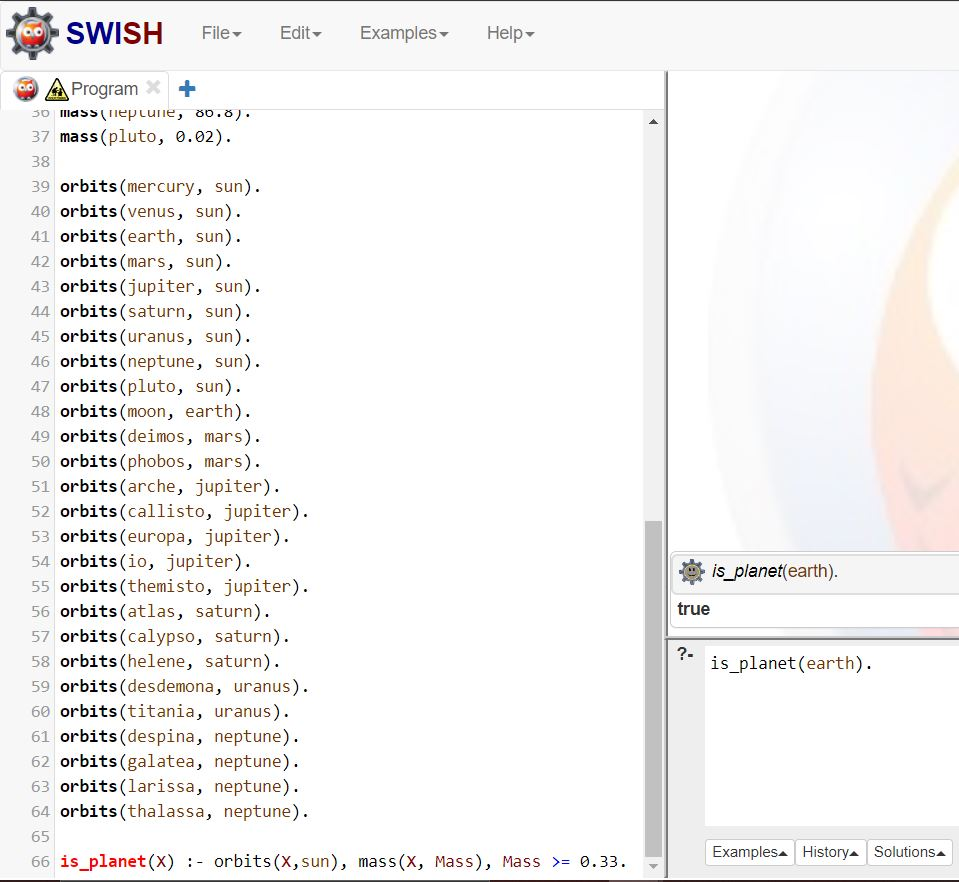
\includegraphics[width=0.75\textwidth]{is-planet_G.JPG}
		\caption{is$\_$planet(earth) - Ground query.}
	\end{figure}
	
	\begin{figure}[htbp]
		\centering
		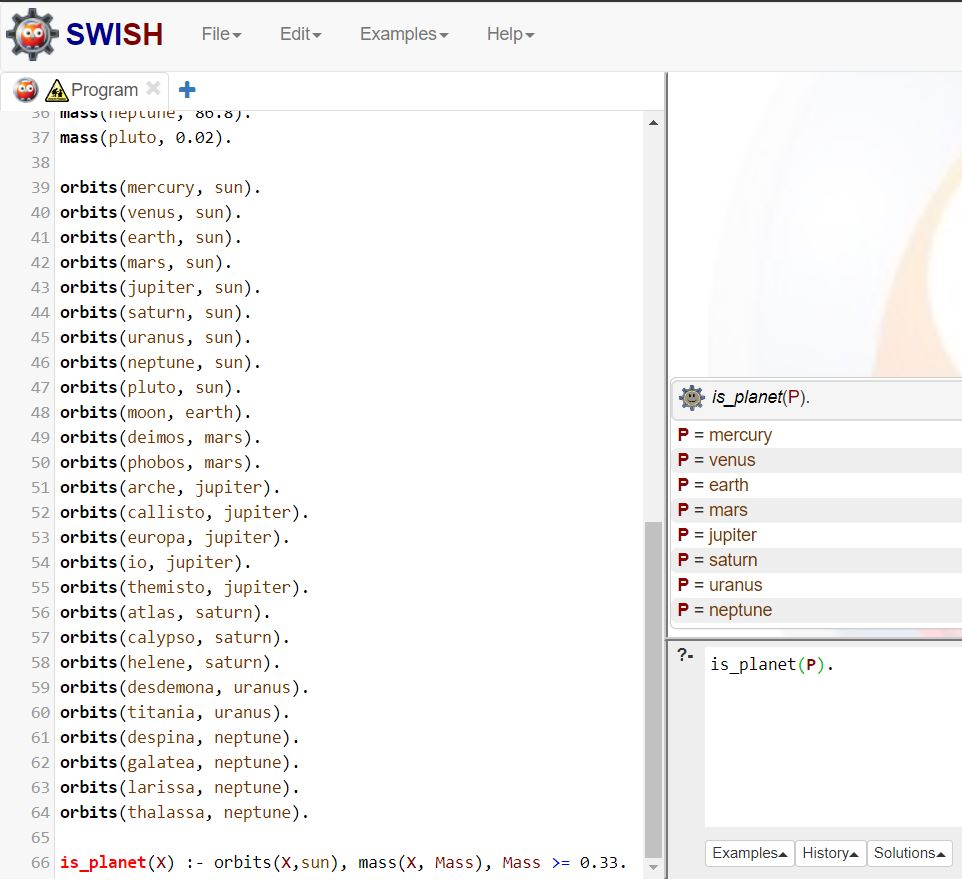
\includegraphics[width=0.75\textwidth]{is-planet_NG.JPG}
		\caption{is$\_$planet(P) - Non-ground query.}
	\end{figure}
	
	\begin{figure}[htbp]
		\centering
		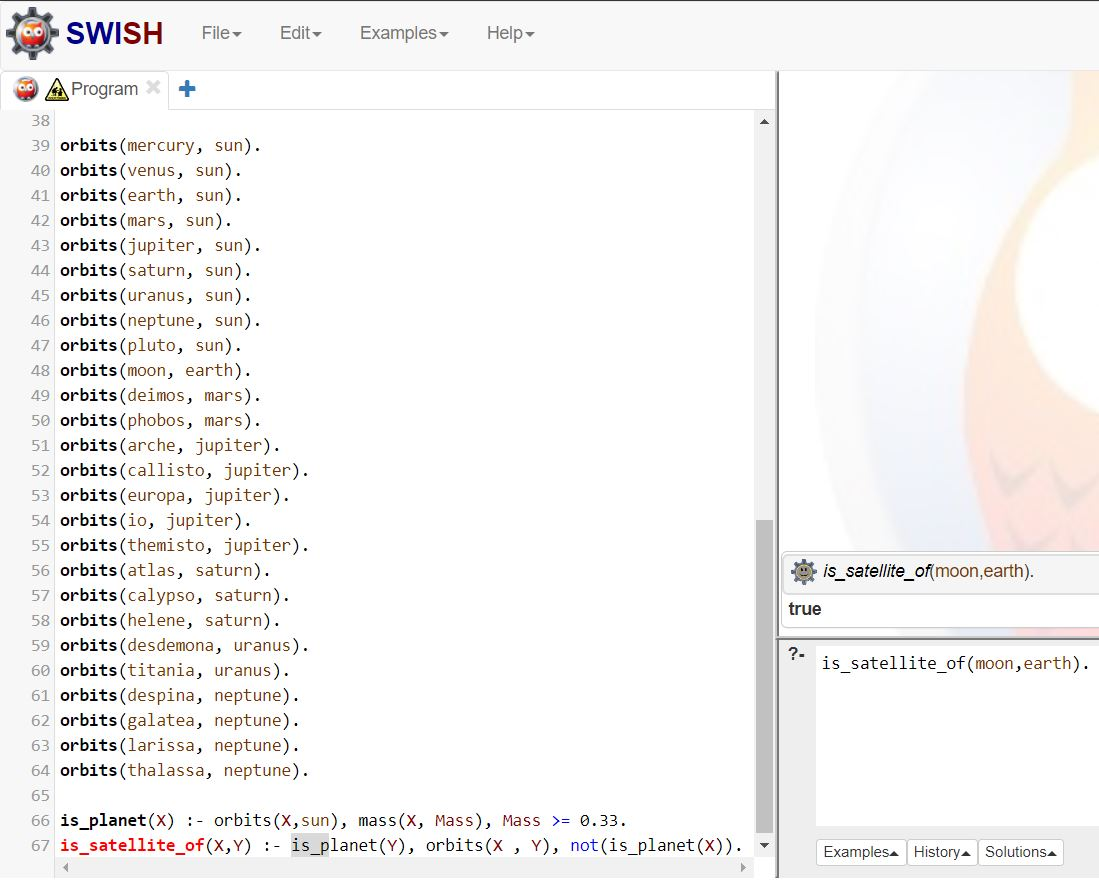
\includegraphics[width=0.75\textwidth]{is-satellite-of_G.JPG}
		\caption{is$\_$satellite$\_$of(moon,earth) - Ground query.}
	\end{figure}
	
	\begin{figure}[htbp]
		\centering
		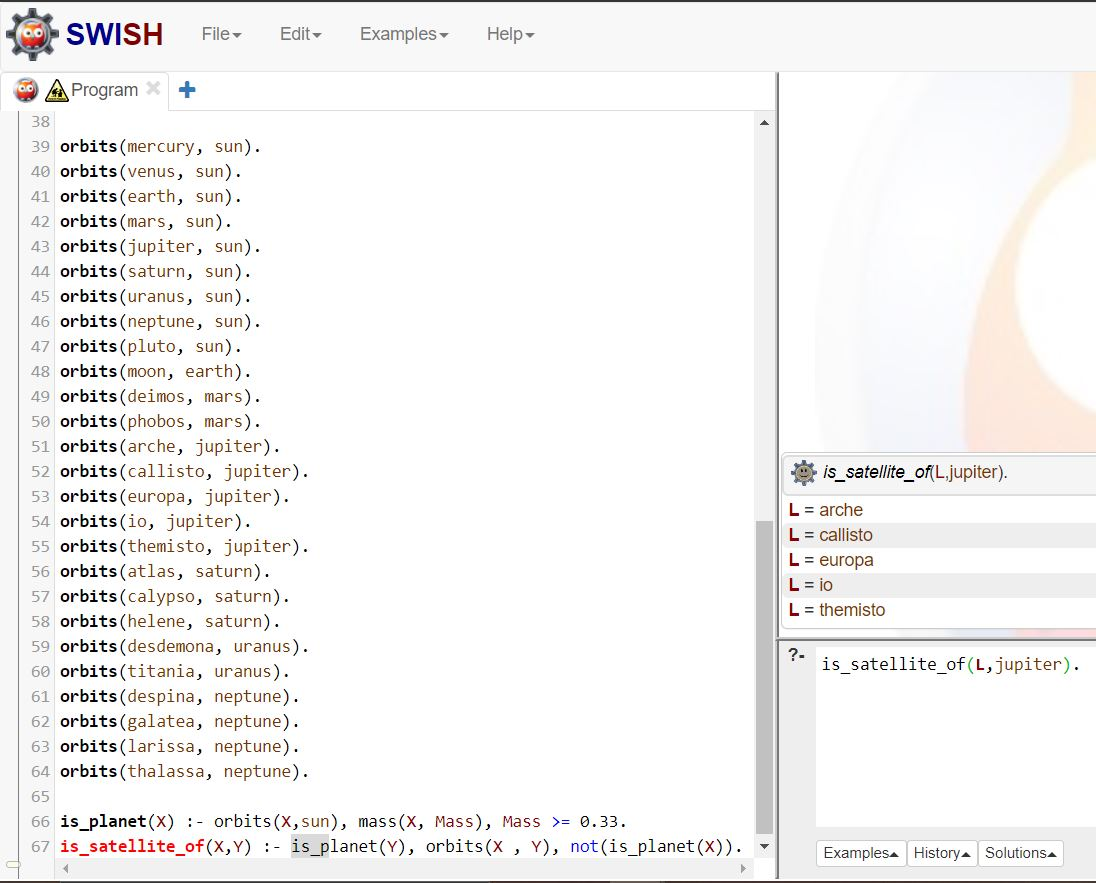
\includegraphics[width=0.75\textwidth]{is-satellite-of_NG.JPG}
		\caption{is$\_$satellite$\_$of(L,jupiter) - Non-ground query.}
	\end{figure}
		
	\begin{figure}[htbp]
		\centering
		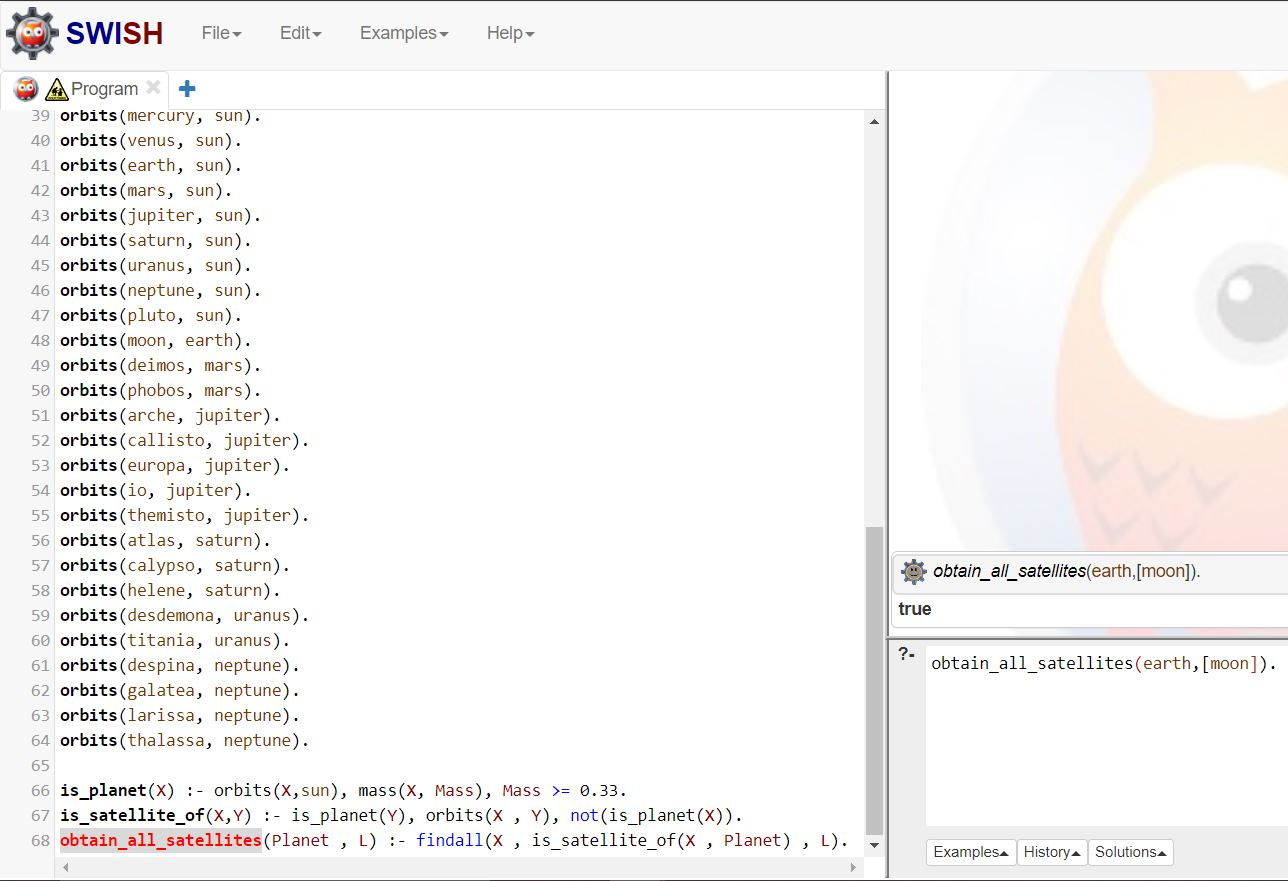
\includegraphics[width=0.75\textwidth]{obtain-all-satellites_G.JPG}
		\caption{obtain$\_$all$\_$satellites$\_$(earth,[moon]) - Ground query.}
	\end{figure}
	
	\begin{figure}[htbp]
		\centering
		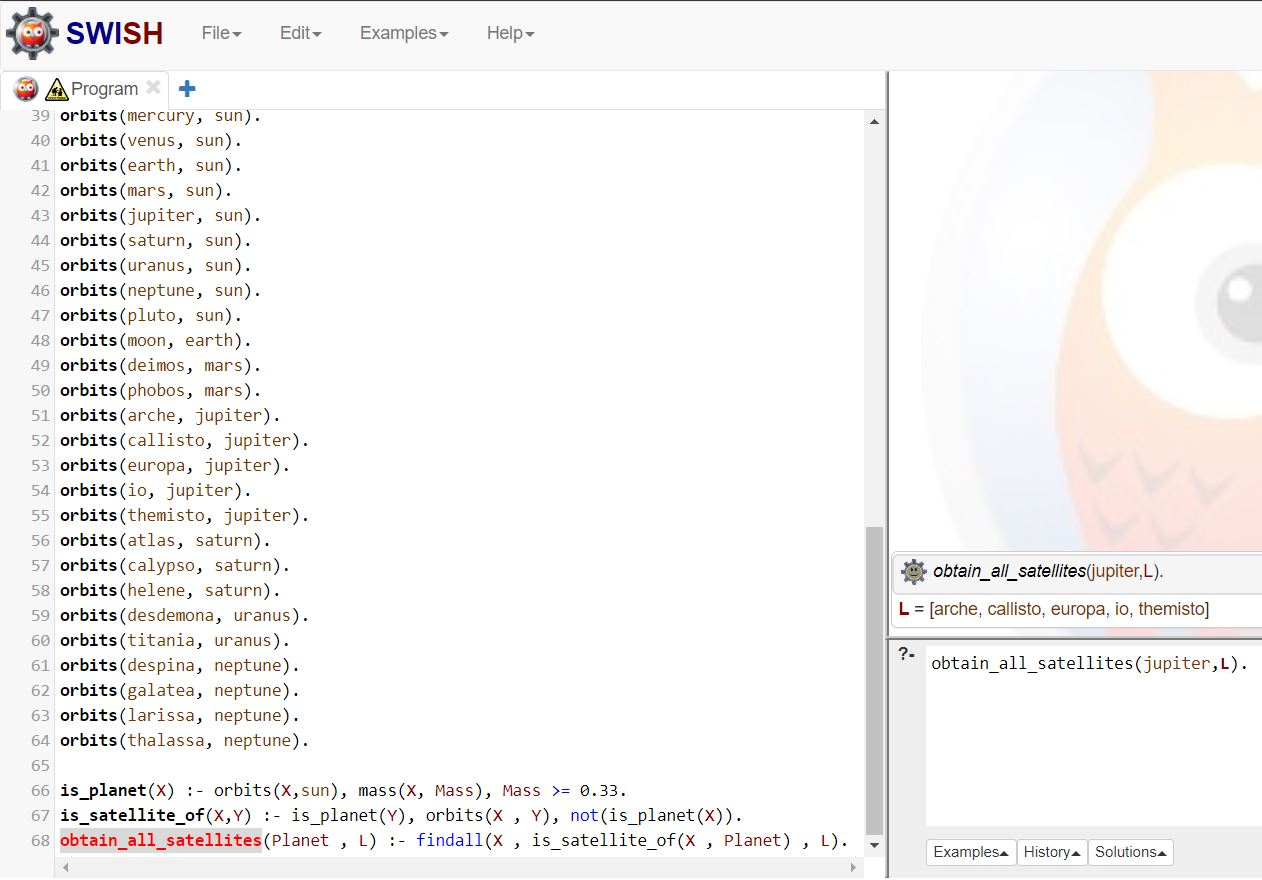
\includegraphics[width=0.75\textwidth]{obtain-all-satellites_NG.JPG}
		\caption{obtain$\_$all$\_$satellites$\_$(jupiter,L) - Non-ground query.}
	\end{figure}
	
\end{enumerate}
\newpage
\newpage
\subsection*{Part 2}

\begin{enumerate}
	\item Type O Particular Negative: $\exists x \neg P(x)$
	
	\item Type A Universal Affirmative: $\forall x P(x)$
	
	\item Type I Particular Affirmative: $\exists x P(x)$
	
	\item Type E Universal Negative: $\forall x \neg P(x)$
\end{enumerate}
\subsection*{Part 3}

\begin{enumerate}
	
	\item The formal definition of Type O categorical propositions is $\exists x \neg P(x)$.
	By negating a type A categorical proposition, and following the laws of logic, we find that:
	
	$\neg (\forall x P(x))$ $\equiv$ $\exists x \neg P(x)$ AND 
	$\neg (\exists x \neg P(x))$ $\equiv$ $\forall x P(x)$
	
	\item The formal definition of Type E categorical propositions is $\forall x \neg P(x)$. In Negating a type E proposition, the universal quantifier($\forall $) becomes the existential quantifier($\exists$) and the proposition is negated. The result yields the type I proposition ($\exists x P(x)$). In the inverse, negating a type I proposition yields a type E proposition.
	
	$\neg (\forall x \neg P(x))$ $\equiv$ $\exists x P(x)$ AND $\neg (\exists x P(x))$ $\equiv$ $\forall x \neg P(x)$.
	\end{enumerate}
\newpage
\section*{Problem 3: Temporal logic}
\subsection*{Part 1}
\begin{enumerate}
	\item Visualization
	\begin{figure}[htbp]
		\centering
		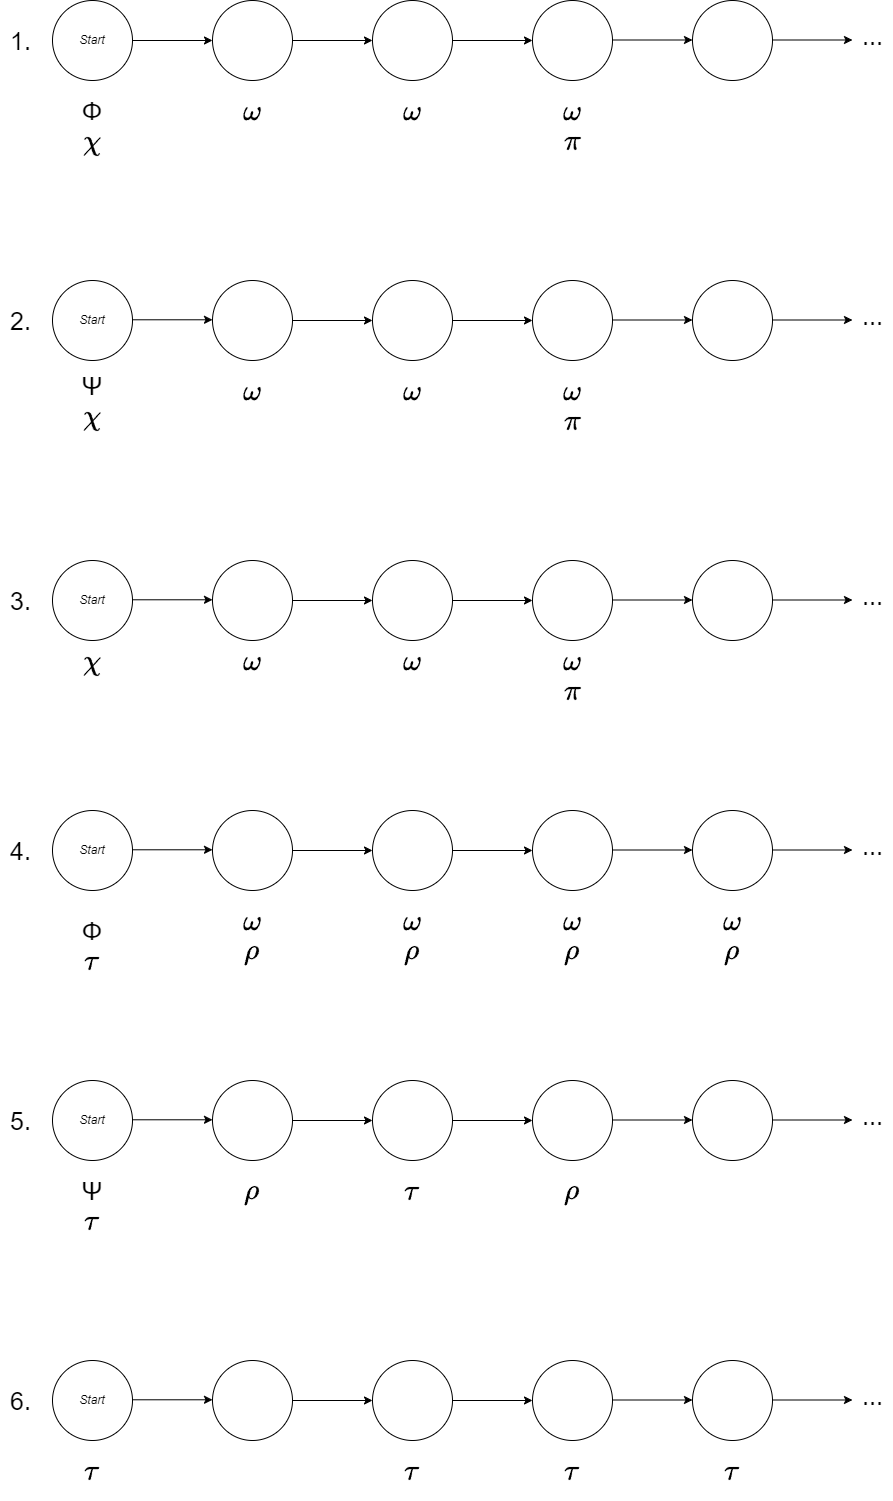
\includegraphics[width=0.60\textwidth]{SOEN331_A1_P311.PNG}
		\caption{Visualization Problem 3}
	\end{figure}
	
	\newpage
	\item In order for the program to terminate, some conditions need to be met depending on the state of the program. If $\omega$ becomes true then for the program to terminate, $\pi$ must also become true at least once after $\omega$. In the case of $\tau$ becoming true then for the program to terminate, $\rho$ must become true after $\tau$. Given any state, the program will terminate eventually.
	 
\end{enumerate}
\subsection*{Part 2}
\begin{enumerate}
	
	\item
	 ($\neg\square\phi$ $\wedge$ $\neg\square\psi$) $\rightarrow$ $\bigcirc\textsuperscript{2}(\lozenge$(x $\mathcal{W}$ $\tau$))
	
	\begin{figure}[htbp]
		\centering
		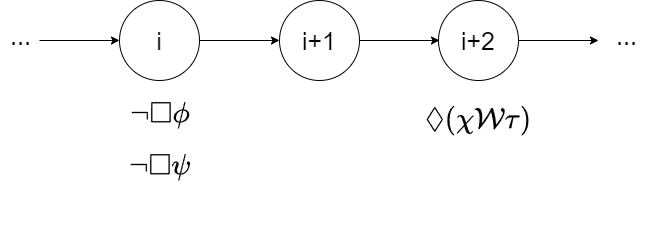
\includegraphics[width=0.60\textwidth]{SOEN331_A1_P321.PNG}
		\caption{Visualization Problem 3 | Part 2 | 1.}
	\end{figure}
	\item If $\alpha$ and $\beta$ do not hold true at the same time then starting the next state, $\gamma$ will eventually hold true until the moment $\delta$ becomes true. $\delta$ is guaranteed to become true.
	\begin{figure}[htbp]
		\centering
		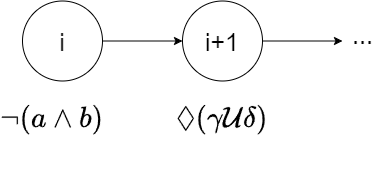
\includegraphics[width=0.40\textwidth]{SOEN331_A1_P322(visual-formula).PNG}
		\caption{Visualization Problem 3 | Part 2 | 2.}
	\end{figure}
	\item If starting at time = i+1, $\tau$ becomes true and $\mathcal{X}$ eventually becomes invariant; Then starting in time = i + 2, $\phi$ becomes true and holds true unless $\psi$ becomes true.
	\begin{figure}[htbp]
		\centering
		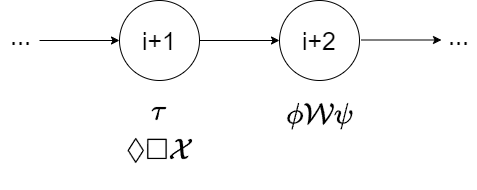
\includegraphics[width=0.50\textwidth]{SOEN331_A1_P323(visual-formula).PNG}
		\caption{Visualization Problem 3 | Part 2 | 3.}
	\end{figure}
\end{enumerate}
\newpage
\section*{Problem 4: Unordered structures}
\begin{enumerate}
	\item $\mathcal{P}Languages$ would be a set containing all possible subsets of Languages, namely the powerset of languages
	\item 
	\begin{enumerate}
		\item Favorites is of type $\mathcal{P}Languages$. This means that Favorites is a non-atomic element, or a subset, of the powerset of the Languages set.
		\item It should be interpreted as a set.
		\item Favorites can be the empty set, any subset of $\mathcal{P}Languages$, or Languages itself.
	\end{enumerate}
	\item
	\begin{enumerate}
		\item Favorites is equal to the entire powerset of the Languages set.
		\item Favorite is a single non-atomic element of the powerset of the Languages set. Not the entire powerset of Languages. Therefore, it is not semantically equivalent.
	\end{enumerate}
	
	\item Having the set $\{$Lua,Groovy,C$\}$ in the power set of Languages would imply that the atomic variables Lua, Groovy and C are contained within the Languages set, which is not the case for Lua.
			This means that $ $\{$Lua,Groovy,C$\}$ \not\in \mathcal{P}Languages$.
	
	\item Yes, because $\{ \{$Lua,Groovy,C$\} \}$ is an element of the powerset of Languages where the superset only contains the element $\{$Lua,Groovy, C$\}$, and not the individual atomic variables.
	\item
	\begin{enumerate}
		\item The variable can be either atomic or non-atomic, depending on what element of Languages it is assigned to. This is because Languages holds both atomic and non-atomic variables.
		\item Non-Atomic. This variable represents a set of elements, since every element in $\mathcal{P}Languages$ is a set.
	\end{enumerate}	
	\item Library: $\mathcal{P}Languages$
	\item No, because the set containing the empty set (‘$\{ \varnothing  \}$’) is not an element of the powerset but the empty set (‘$\{ \}$’ or '$\varnothing$') would be.
	\item Refer to problem4-9.lsp in /code
\end{enumerate}
\section*{Problem 5: Ordered structures}
\begin{enumerate}
	\item 
	
	\begin{tabbing}
		\hspace{0.5pt}\=
		\\ % Adjust the width of the tab here
		\>Enqueue(Q, T): \hspace{0.5pt}\=\\
		\>\> $\Sigma$1' = cons(T , $\Sigma$1) \\
		\\
		\>Dequeue(Q): \\
		\>\> while $\Sigma$1 is not empty:\hspace{0.5pt}\= \\
		\>\>\> $\Sigma$2' = cons(head($\Sigma$1) , $\Sigma$2) \\
		\>\>\> $\Sigma$1’ = tail($\Sigma$1) \\
		\>\> x = head($\Sigma$2) \\
		\>\> while $\Sigma$2 is not empty:\hspace{0.5pt}\= \\
		\>\>\> $\Sigma$1' = cons(head($\Sigma$2) , $\Sigma$1) \\
		\>\>\> $\Sigma$2’ = tail($\Sigma$2) \\
		\>\>Return x
	\end{tabbing}
	
	\item Refer to file queue-adt.lsp in /code
	\item Refer to file problem5-3.pl in /code
\end{enumerate}
\section*{Problem 6: Binary relations, functions and orderings}
\subsection*{Part 1}
\begin{enumerate}
	\item
	Given binary relation R : “is of type” in the domain of types in the Java API, we find that:\newline
	1 - R is reflexive, $\forall$a $\in$A : aRa, meaning for any type a, a is of type a. This is true because, in the Java API, any type is considered to be a type of itself;
	
	2 - R is anti-symmetric, $\forall$a, b $\in$ A : (aRb $\wedge$ bRa) → a = b, meaning for any type a and b, if a is of type b and b is of type, then a = b. In the Java API, for an element to be of a specific type, it must be an element of that type, or an element of a subtype of that type. This means that for two types to be types of each other, they must be the same type.
	
	3 - R is transitive, $\forall$a, b, c $\in$ A : (aRb $\wedge$ bRc) → aRc, meaning for any type a, b and c, if a is of type b, and b is of type c, then a is of type c. As stated previously, for an element to be of a specific type, it must be an element of that type, or an element of a subtype of that type. So, if a is of type b, and b is of type c, we can come to the conclusion that a is of type c.
	
	Therefore, we find that R is a partial order.
	\item
	Given the set of vertices V1 and edges E, we can prove that (V1, R) is a poset:
	
	1 - From the given edges, there are explicit examples of the reflexive property. However, in the Java API context, reflexivity is implied, as any type is considered to be a type of itself.
	
	2 - In the given edges, there are no examples of two types relating to each other, and not being the same type, therefore, the conditions for anti-symmetry are satisfied.
	
	3 - Given the context of the Java API, (\(V_1\),R) can be considered transitive because of inheritance. For example, in the given edges, we find that NavigableMap is of type SortedMap, and that SortedMap is of type Map, therefore, considering the context, NavigableMap is also of type Map.
	
	\item Hasse Diagram of (\(V_1,R\))
	\begin{figure}[htbp]
		\centering
		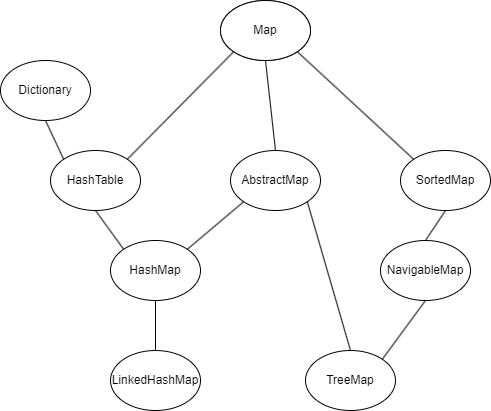
\includegraphics[width=0.60\textwidth]{SOEN331_A1_P613.PNG}
		\caption{Visualization Problem 6.1.3}
	\end{figure}
	
\end{enumerate}
\subsection*{Part 2}
\begin{enumerate}
	\item 
	1 - The binary relation is subset of is reflexive, $\forall$a $\in$ A : aRa, since every set is a subset of itself.
	
	2 - It is antisymmetric, $\forall$a, b $\in$ A : (aRb $\wedge$ bRa) → a = b, since any two sets that are subsets of each other must be the same set.
	
	3 - It is also transitive, $\forall$a, b, c $\in$ A : (aRb $\wedge$ bRc) → aRc, because if a set \(S_1\) is a subset of a set \(S_2\), and \(S_2\) is a subset that a set \(S_3\), then \(S_1\) is a subset of \(S_3\).
	For example, \(S_1\) = $\{1 , 2\}$, \(S_2\) = $\{1 , 2 , 3\}$ and \(S_3\) = $\{1 , 2 , 3 , 4\}$, \(S_1\) is a subset of \(S_2\), and \(S_2\) is a subset of \(S_3\), and \(S_1\) is also a subset of \(S_3\).
	
	\item
	P(\(V_2\)) = $\{\{\} , \{a\} , \{b\} , \{c\} , \{a,b\} , \{a,c\} , \{b,c\} \{a,b,c\}\}$
	
	1 - The power set of \(V_2\) is indeed reflexive since all sets within P(\(V_2\)) are subsets of themselves.
	
	2 - It is anti-symmetric since there are no 2 distinct elements that are subsets of each other, or (a, b) $\in$ A $\wedge$ a $\neq$ b $\rightarrow$ (b, a) $\not\in$ R.
	
	3 - It is transitive since $\forall$a, b, c $\in$ A : (aRb $\wedge$ bRc) $\rightarrow$ aRc. This can be seen in P(\(V_2\)) from $\{a\}$ , $\{a,b\}$ and $\{a,b,c\}$, where $\{a\}$ is a subset of both $\{a,b\}$ and $\{a,b,c\}$, and $\{a,b\}$ is a subset of $\{a,b,c\}$.

	\item Hasse Diagram of \((P(V_2) , \subseteq)\)
	\begin{figure}[htbp]
		\centering
		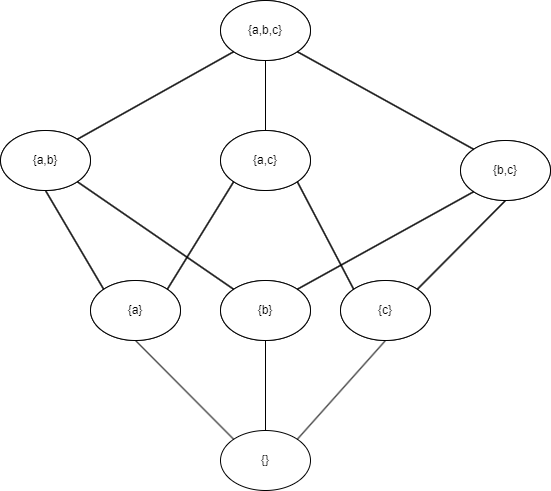
\includegraphics[width=0.60\textwidth]{SOEN331_A1_P623.PNG}
		\caption{Visualization Problem 6.2.3}
	\end{figure}

	Minimal Values: \(\{\{\}\}\).\\
	Maximal Values: \(\{a,b,c\}\).
\end{enumerate}
\subsection*{Part 3}
\begin{enumerate}
	\item - Map is indeed a function, since every element in the domain maps to at most 1 element in the co-domain.
	
	\item - It is a partial function, since not every element in the domain participated in the mapping. 		map : V1 $\not\rightarrow$ P(\(V_2\))
	
	\item - It is not injective since some elements in the co-domain are mapped to twice, namely $\{a ,b ,c\}$. The definition for an injective function is $\forall$x, y $\in$ V1 : x $\neq$ y → f (x) $\neq$ f (y), which is not followed in this case.
	
	\item - It is not surjective since not every element in the co-domain is mapped to by at least one element in the domain. The definition for a surjective function is $\forall$z $\exists$ P(\(V_2\)), $\exists$x $\in$ V1 : f (x) = z, which is not the case.
	
	\item - Since the function is neither injective nor surjective, it is not bijective.
	
	\item -  The function is order-preserving since all predecessor relationships between elements in the domain are preserved by their images in the codomain. In other words 
	x $\prec$ y in V1 implies f (x) $\prec$ f (y) in P(\(V_2\)). In this case, we have NavigableMap → {c} and TreeMap → $\{\}$, where TreeMap $\prec$ NavigableMap in V1 implies {} $\prec$ {c} in P(\(V_2\)).
	
	\item - The function is not order-preserving since not all predecessor relationships between elements in the codomain are reflected by their pre-images in the domain. In other words, we say a function is order reflecting if f (x) $\prec$ f (y) in P(\(V_2\)) implies x $\prec$ y in V1. In this case, we have $\{c\}$ $\prec$ $\{a,b,c\}$ , which is not reflected by the images, meaning we don’t have NavigableMap $\prec$ AbstractMap.
	
	\item - The function is not order-embedding since it is not both order-preserving and order-reflecting.
	
	\item -  The function is not isomorphic since it is neither order-embedding nor surjective.
\end{enumerate}


\section*{Problem 7: Construction techniques}
\begin{enumerate}
	\item 
	\begin{verbatim}
		compress (T) is
			comp_list = ⟨⟩
			for all i in T
				if(head(comp_list) != i)
					consR(com_list, i)
			return comp_list
	\end{verbatim}

	\item
	\begin{verbatim}
		compress (T) is
			if(T = ⟨⟩) then
				return ⟨⟩
			if(head(T) = head(tail(T))) then
				return compress(tail(T))
			else
				return cons(head(T), compress(tail(T)))
	\end{verbatim}
	
	\item 
	\begin{verbatim}
	compress(⟨a, a, b, b, c, a⟩) = compress(⟨a,b,b,c,a⟩)
								= cons(a, compress(⟨b,b,c,a⟩))
								= cons(a, compress(⟨b,c,a⟩))
								= cons(a, cons(b, compress(⟨c,a⟩)))
								= cons(a, cons(b, cons(c, compress(⟨a⟩))))
								= cons(a, cons(b, cons(c, cons(a, compress(⟨⟩)))))
								= cons(a, cons(b, cons(c, cons(a, ⟨⟩))))
								= cons(a, cons(b, cons(c, ⟨a⟩)))
								= cons(a, cons(b, ⟨c ,a⟩))
								= cons(a, ⟨b ,c ,a⟩)
								= ⟨a, b ,c ,a⟩
	\end{verbatim}
	
	\item Refer to file compress.lsp in /code
	
\end{enumerate}


\end{spacing}
\end{document}
